% Author: Izaak Neutelings (June, 2018)
\documentclass[border=3pt,tikz]{standalone}
\usepackage{ifthen}
\usepackage{siunitx}
\usepackage{tikz}
\usetikzlibrary{hobby} % for ..
\usetikzlibrary{arrows.meta} % to control arrow size
\tikzset{>={Latex[length=4,width=4]}} % for LaTeX arrow head
\usetikzlibrary{calc,intersections,decorations.markings}
\usepackage{siunitx}
\usepackage{xcolor} % for colored text

\colorlet{mylightblue}{blue!20}
\colorlet{myblue}{blue!50!black}
\colorlet{mydarkblue}{blue!30!black}
\colorlet{mylightred}{red!10}
\colorlet{myred}{red!50!black}
\colorlet{mydarkred}{red!60!black}
\colorlet{mydarkgreen}{green!30!black}

%\tikzstyle{midarr}=[decoration={markings,mark=at position 0.5 with {\arrow{stealth}}},postaction={decorate}]
\tikzset{
  midarr/.style={decoration={markings,mark=at position #1 with {\arrow{stealth}}},postaction={decorate}},
  midarr/.default=0.5
}
\def\tick#1#2{\draw[thick] (#1) ++ (#2:0.03*\ymax) --++ (#2-180:0.06*\ymax)}

\begin{document}


% PV diagram - van der Waals isotherms
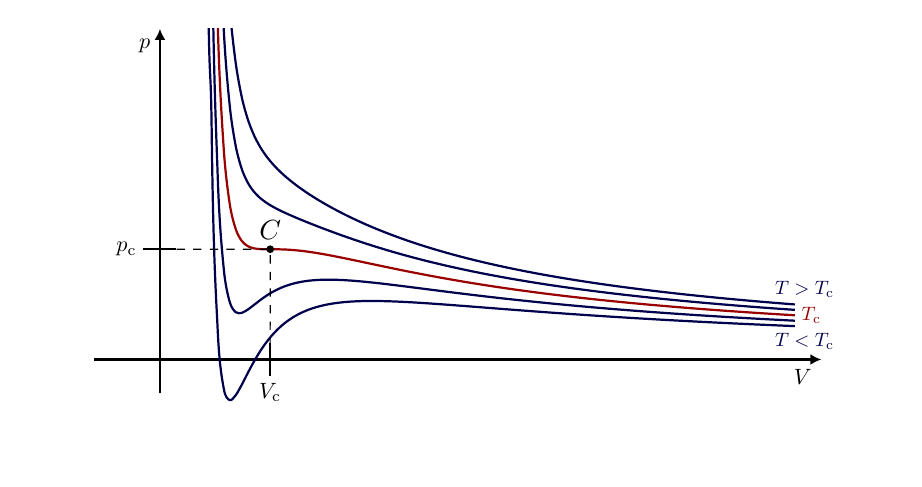
\begin{tikzpicture}[scale=1.4]
  \message{PV diagram - van der Waals isotherms^^J}
  \def\tick{0.05*\xmax}
  \def\xmax{6}
  \def\ymax{3}
  \def\N{100}
  \def\s{1}
  \def\R{4}
  \def\isotherm#1#2{{ (8*#2)/(3*#1-1) - 3/(#1*#1) }} % reduced equation of state
  \coordinate (C) at (\s,1);
  
  % AXIS
  \draw[->,thick] (0,-0.1*\ymax) -- (0,\ymax)
    node[anchor=north east,inner sep=4,scale=0.8] {$p$};
  \draw[->,thick] (-0.1*\xmax,0) -- (\xmax,0)
    node[anchor=north east,inner sep=4,scale=0.8] {$V$};
  
  % ISOTHERMS
  \begin{scope}
    \clip (-0.2*\xmax,-0.3*\ymax) rectangle (1.11*\xmax,\ymax);
    \foreach \i/\T in {1/0.8,2/0.9,3/1.0,4/1.1,5/1.2}{
      \ifthenelse{\lengthtest{\T pt = 1.0 pt}}{
        \draw[mydarkred,thick,variable=\x,domain=0.36:{.96*\xmax/\s},range=0:1,samples=\N,smooth]
          plot (\s*\x,\isotherm{\x}{\T}) coordinate (EC);
      }{
        \draw[mydarkblue,thick,variable=\x,domain=0.36:{.96*\xmax/\s},range=0:1,samples=\N,smooth]
          plot (\s*\x,\isotherm{\x}{\T}) coordinate (E\i);
      }
    }
  \end{scope}
  
  % LABELS
  \node[mydarkblue,scale=0.7,right=5,below] at (E1) {$T<T_\text{c}$};
  \node[mydarkred,right,scale=0.7] at (EC) {$T_\text{c}$};
  \node[mydarkblue,scale=0.7,right=5,above] at (E5) {$T>T_\text{c}$};
  
  % CRITICAL POINT
  \fill[black] (C) circle (1pt) node[above]{$C$};
  \draw[dashed] (0,1) -- (C) -- (\s,0);
  \draw[thick] (\s,\tick/2) --++ (0,-\tick) node[below=-.5pt,scale=0.8] {$V_\text{c}$};
  \draw[thick] (\tick/2,1) --++ (-\tick,0) node[left=-.5pt,scale=0.8] {$p_\text{c}$};
  
  
\end{tikzpicture}


\end{document}